% Szglab4
% ===========================================================================
%

\newcounter{enumi_saved}

\newcommand{\breaktable}{%
 \setcounter{enumi_saved}{\value{enumi}}
 \end{itemize}\end{itemize}\\
 \begin{itemize}\begin{itemize}
 \setcounter{enumi}{\value{enumi_saved}}
}

\chapter{Szkeleton tervezése}

\thispagestyle{fancy}

\section{Errata}

Az előző fejezetben leírtak egy apró részletben megváltoztak. Az elemeket már nem közvetlenül kötjük össze, hanem \textit{vezeték}ek segítségével, melyeket egymással \textit{csomópont}okkal lehet összekötni, ha szükséges. Így javítottuk a láthatósággal kapcsolatosan felmerült problémákat, ehhez fel kellett venni 2 új osztályt (Wire, Node), illetve az AbstractComponent módosítani, ezekhez tartozó objektum és osztályleírások alább olvashatóak, valamint mellékeltük a módosított statikus osztálydiagramot is. (Egy-két egyéb objektumleírás is módosult, de csak azért mert a kiértékelés logikája változott -- nem hátulról megyünk, hanem az összes kiértékeli magát, ez nem szükséges a jelen fejezethez, hiszen magától értetődő)

\subsection{Objektumleírás: \bf Wire}
Vezeték, mely az áramköri komponensek ki és bemeneteit köti össze. Egy vezeték egy darab kimenetet és egy darab bemenetet köt össze. A rajta lévő értéket le lehet tőle kérdezni, illetve be lehet azt állítani.

\subsection{Objektumleírás: \bf Node}
Csomópont, mely a bemenetén lévő értéket a kimeneteire adja. Segítségével lehet egy vezetéket ,,szétágaztatni''.

\subsection{Osztályleírás: \bf AbstractComponent}
Absztrakt osztály.
\begin{itemize}
\item Felelősség\\
Egy komponens absztrakt megvalósítása, ebből származik az összes többi  komponens. A közös logikát valósítja meg. A gyakran használt feladatokra ad alapértelmezett implementációt (pl. vezetékek bekötése). Tudja magáról, hogy a legutóbbi két kiértékelés között változtak-e a kimenetei.
\item Ősosztályok: (nincs)
\item Interfészek: (nincs)
\item Attribútumok $\ $
\begin{itemize}
	\item \texttt{protected Wire[] inputs}: Bemeneteire kötött vezetékek.
	\item \texttt{protected Wire[] outputs}: Kimeneteire kötött vezetékek.
\end{itemize}
\item Metódusok$\ $
\begin{itemize}
	\item \texttt{addTo(Circuit c)}: Meghívja az áramkör \texttt{add(AbstractComponent ac)} metódusát.
	\item \texttt{void evaluate()}: Komponens kimenetein lévő értékek kiszámolása a bemenetek alapján.
	\item \texttt{boolean isChanged()}: Visszaadja, hogy a legutóbbi két kiértékelés között változtak-e a kimenetek.
	\item \texttt{void setInput(int inputPin, Wire wire)}: Az adott bemeneti lábára rákötjük a megadott vezetéket.
	\item \texttt{void setOutput(int outputPin, Wire wire)}: Az adott kimeneti lábára rákötjük a megadott vezetéket.
\end{itemize}
\end{itemize}

\subsection{Osztályleírás: \bf Node}
\begin{itemize}
\item Felelősség\\
Csomópont, mely a bemenetén lévő értéket a kimeneteire adja. Segítségével lehet egy vezetéket ,,szétágaztatni''.
\item Ősosztályok:\ AbstractComponent.
\item Interfészek: (nincs)
\item Attribútumok $\ $
\begin{itemize}
\item (nincs)
\end{itemize}
\item Metódusok$\ $
\begin{itemize}
\item (nincs)
\end{itemize}
\end{itemize}

\subsection{Osztályleírás: \bf Wire}
\begin{itemize}
\item Felelősség\\
Vezeték, mely az áramköri komponensek ki és bemeneteit köti össze. Egy vezeték egy darab kimenetet és egy darab bemenetet köt össze. A rajta lévő értéket le lehet tőle kérdezni, illetve be lehet azt állítani.
\item Ősosztályok:\ AbstractComponent.
\item Interfészek: (nincs)
\item Attribútumok $\ $
\begin{itemize}
	\item \texttt{private Value value}: Vezetéken lévő érték
\end{itemize}
\item Metódusok$\ $
\begin{itemize}
	\item \texttt{Value getValue()}: Visszaadja a vezetéken lévő értéket.
	\item \texttt{void setValue(Value v)}: Beállítja a vezetéken lévő értéket.
\end{itemize}
\end{itemize}

\subsection{Statikus struktúra diagramok}

\begin{figure}[H]
\begin{center}
\includegraphics*[angle=90, width=17cm, viewport = 25 30 705 565]{chapters/chapter04/classdiagram/class.pdf}
\caption{Statikus struktúra nézet}
\label{fig:class_diagram}
\end{center}
\end{figure}

\section{A szkeleton modell valóságos use-case-ei}

\subsection{Use-case diagram}

\begin{figure}[h]
\begin{center}
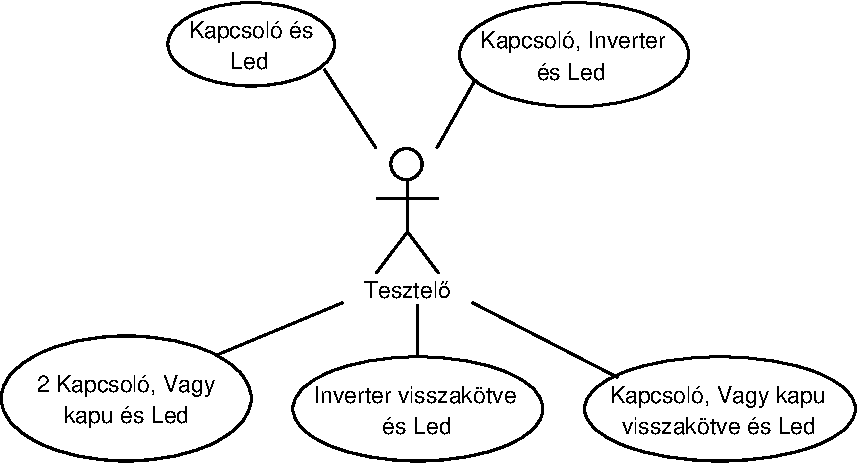
\includegraphics[width=10cm]{chapters/chapter05/imgs/usecase.pdf}
\caption{A szkeleton modell valóságos use-case-ei}
\label{fig:SzkeletonUseCase}
\end{center}
\end{figure}

\subsection{Use-case leírások}

Lenti use-caseknél, ahol valamilyen információ szerint dönteni kell, vagy csak szükségünk van a skeleton jellegéből adódó hiányzó információkra, azt a felhasználótól kérjük be. Ahhoz, hogy a szekvenciadiagramokon lévő szekvenciákat kapjunk, a javasolt értéket kell beírnia a tesztelőnek.\\

Nem akartuk, hogy az áramkör inicializálása minden use-casenél ott legyen, ezzel elfedve a lényegi részeket, ezért ezt egy külön use-case-ben bemutatjuk, a többinél csak jelezzük, hogy ott is van ilyen lépés. A tesztelő, majd egy adott tesztesetnél választhat, hogy kíváncsi-e az inicializálásra vagy sem.

\usecase
{Áramkör inicializálása}
{Ez a usecase egy áramkör és a hozzá tartozó szimuláció inicializálását mutatja be, hogyan jönnek létre a komponensek és a közöttük lévő összeköttetés. Jelen példa egy Kapcsoló és egy Led összeköttetését prezentálja.}
{Tesztelő}
{\vspace{-15pt}
\begin{itemize}
\setlength{\itemsep}{0cm}%
\setlength{\parskip}{0cm}%
\item szimuláció létrehozása
\item áramkör létrehozása
\item áramkör beregisztrálása a szimulációba
\item áramkör inicializálása
\begin{itemize}
\setlength{\itemsep}{0cm}%
\setlength{\parskip}{0cm}%
	\item kapcsoló létrehozása
	\item vezeték létrehozása
	\item kapcsoló kimenetére vezeték kötése
	\item led létrehozása
	\item led bemenetére vezeték kötése
	\item kapcsoló áramkörbe regisztrálása
	\item led áramkörbe regisztrálása
\end{itemize}
\end{itemize}
\vspace{-15pt}}

\newpage

\usecase
{Kapcsoló és Led}
{Ez a usecase egy olyan áramkör tesztelését mutatja be, amely egy kapcsolóból és rá kötött ledből áll.\newline
\begin{center}
\vspace{-15pt}
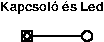
\includegraphics[scale=1.5]{dw/circuit_test1.pdf}
\vspace{-10pt}
\end{center}
}
{Tesztelő}
{\vspace{-15pt}
\begin{itemize}
\setlength{\itemsep}{0cm}%
\setlength{\parskip}{0cm}%
\item Áramkör és komponensek létrehozása
%\begin{itemize}
%\setlength{\itemsep}{0cm}%
%\setlength{\parskip}{0cm}%
%\item áramkör létrehozása
%\item áramkör beregisztrálása a szimulációba
%\item vezeték létrehozása
%\item kapcsoló létrehozása
%\item kapcsoló kimenetére vezeték kötése
%\item led létrehozása
%\item led bemenetére vezeték kötése
%\item kapcsoló áramkörbe regisztrálása
%\item led áramkörbe regisztrálása
%\end{itemize}
\item szimuláció indítása
\begin{itemize}
\setlength{\itemsep}{0cm}%
\setlength{\parskip}{0cm}%
\item hálózat kiértékelés indítása
\begin{itemize}
\setlength{\itemsep}{0cm}%
\setlength{\parskip}{0cm}%
	\item kapcsoló kiértékelése
	\begin{itemize}
	\setlength{\itemsep}{0cm}%
	\setlength{\parskip}{0cm}%
		\item kapcsoló állapotának lekérdezése (\textbf{megkérdezi a tesztelőt}, javasolt: 1)
		\item kapcsoló értékének kiadása a vezetékre
	\end{itemize}
	\item led kiértékelése
	\begin{itemize}
	\setlength{\itemsep}{0cm}%
	\setlength{\parskip}{0cm}%
		\item led bemenetének lekérdezése (\textbf{megkérdezi a tesztelőt}, javasolt: 1)
	\end{itemize}
\end{itemize}
\item áramkör változásának vizsgálata
\begin{itemize}
\setlength{\itemsep}{0cm}%
\setlength{\parskip}{0cm}%
	\item kapcsoló változásának vizsgálata (\textbf{megkérdezi a tesztelőt}, javasolt: 1)
	\item led változásának vizsgálata (\textit{idáig nem kéne eljutni, ha fent jót válaszolt a tesztelő})
\end{itemize}
\item áramkör változott, ezért új ciklus
\item hálózat kiértékelés indítása
\begin{itemize}
\setlength{\itemsep}{0cm}%
\setlength{\parskip}{0cm}%
	\item \textit{ugyanazon lépések történnek mint az előző kiértékelésnél, és ugyanazon válaszokat javasolt adni.}
\end{itemize}
\item áramkör változásának vizsgálata
\begin{itemize}
\setlength{\itemsep}{0cm}%
\setlength{\parskip}{0cm}%
	\item kapcsoló változásának vizsgálata (\textbf{megkérdezi a tesztelőt}, javasolt: 0)
	\item led változásának vizsgálata (\textbf{megkérdezi a tesztelőt}, javasolt: 0)
\end{itemize}
\item áramkör nem változott, stabil állapot
\item FF-okat véglegesítjük (nem történik semmi, mert nincs FF)
\item jelgenerátorokat léptetjük (nem történik semmi, mert nincs jelgenerátor)
\item szimuláció vége
\end{itemize}
\end{itemize}
\vspace{-15pt}}

\newpage

\usecase
{Kapcsoló, Inverter és Led}
{Ez a usecase egy olyan áramkör tesztelését mutatja be, amely egy kapcsolóból egy rá kötött inverterből és egy arra kötött ledből áll.\newline
\begin{center}
\vspace{-15pt}
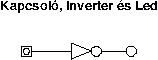
\includegraphics[scale=1.5]{dw/circuit_test2.pdf}
\vspace{-10pt}
\end{center}}
{Tesztelő}
{\vspace{-15pt}
\begin{itemize}
\setlength{\itemsep}{0cm}%
\setlength{\parskip}{0cm}%
\setlength{\itemindent}{-10pt}%
\item Áramkör és komponensek létrehozása
%\begin{itemize}
%\setlength{\itemsep}{0cm}%
%\setlength{\parskip}{0cm}%
%\item áramkör létrehozása
%\item áramkör beregisztrálása a szimulációba
%\item vezeték létrehozása a kapcsoló és az inverter összekötéséhez
%\item kapcsoló létrehozása
%\item kapcsoló kimenetére vezeték kötése
%\item inverter létrehozása
%\item inverter bemenetére vezeték kötése
%\item vezeték lérehozása az inverter és a led összekötéséhez
%\item inverter kimenetére vezeték kötése
%\item led létrehozása
%\item led bemenetére vezeték kötése
%\item kapcsoló áramkörhöz adása
%\item led áramkörhöz adása
%\item inverter áramkörhöz adása
%\end{itemize}
\item szimuláció indítása
\begin{itemize}
\setlength{\itemsep}{0cm}%
\setlength{\parskip}{0cm}%
\setlength{\itemindent}{-25pt}%
\item hálózat kiértékelés indítása
\begin{itemize}
\setlength{\itemsep}{0cm}%
\setlength{\parskip}{0cm}%
\setlength{\itemindent}{-25pt}%
	\item kapcsoló kiértékelése
	\begin{itemize}
	\setlength{\itemsep}{0cm}%
	\setlength{\parskip}{0cm}%
	\setlength{\itemindent}{-35pt}%
		\item kapcsoló állapotának lekérdezése (\textbf{megkérdezi a tesztelőt}, javasolt: 1)
		\item kapcsoló értékének kiadása a vezetékre
	\end{itemize}
	\item inverter kiértékelése
	\begin{itemize}
	\setlength{\itemsep}{0cm}%
	\setlength{\parskip}{0cm}%
	\setlength{\itemindent}{-35pt}%
		\item bemenet lekérdezése (\textbf{megkérdezi a tesztelőt}, javasolt: 1)
		\item kimenet kiadása a vezetékre (\textbf{megkérdezi a tesztelőt}, javasolt: 0)
	\end{itemize}\item led kiértékelése
	\begin{itemize}
	\setlength{\itemsep}{0cm}%
	\setlength{\parskip}{0cm}%
	\setlength{\itemindent}{-35pt}%
		\item led bemenetének lekérdezése (\textbf{megkérdezi a tesztelőt}, javasolt: 0)
	\end{itemize}
\end{itemize}
\item áramkör változásának vizsgálata
\begin{itemize}
\setlength{\itemsep}{0cm}%
\setlength{\parskip}{0cm}%
\setlength{\itemindent}{-25pt}%
	\item kapcsoló változásának vizsgálata (\textbf{megkérdezi a tesztelőt}, javasolt: 1)
	\item inverter változásának vizsgálata (\textit{idáig nem kéne eljutni, ha fent jót válaszolt a tesztelő})
	\item led változásának vizsgálata (\textit{idáig nem kéne eljutni, ha fent jót válaszolt a tesztelő})
\end{itemize}
\item áramkör változott, ezért új ciklus
\item hálózat kiértékelés indítása
\begin{itemize}
\setlength{\itemsep}{0cm}%
\setlength{\parskip}{0cm}%
\setlength{\itemindent}{-25pt}%
	\item \textit{ugyanazon lépések történnek mint az előző kiértékelésnél, és ugyanazon válaszokat javasolt adni.}
\end{itemize}
\item áramkör változásának vizsgálata
\begin{itemize}
\setlength{\itemsep}{0cm}%
\setlength{\parskip}{0cm}%
\setlength{\itemindent}{-25pt}%
	\item kapcsoló változásának vizsgálata (\textbf{megkérdezi a tesztelőt}, javasolt: 0)
	\item inverter változásának vizsgálata (\textbf{megkérdezi a tesztelőt}, javasolt: 0)
	\item led változásának vizsgálata (\textbf{megkérdezi a tesztelőt}, javasolt: 0)
\end{itemize}
\item áramkör nem változott, stabil állapot
\item FF-okat véglegesítjük (nem történik semmi, mert nincs FF)
\item jelgenerátorokat léptetjük (nem történik semmi, mert nincs jelgenerátor)
\item szimuláció vége
\end{itemize}
\end{itemize}
\vspace{-15pt}}

\newpage

	\begin{longtable}{| l | p{12cm} |}
	\hline
	\textbf{Use-case neve}   & {2 Kapcsoló, Vagy kapu és Led} \tabularnewline
	\hline\hline
	Rövid leírás    & {Ez a usecase egy olyan áramkör tesztelését mutatja be, amely egy vagy kapura kötött két kapcsolóból és a vagy kapu kimenetére kötött ledből áll.\newline
\begin{center}
\vspace{-15pt}
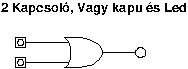
\includegraphics[scale=1.5]{dw/circuit_test3.pdf}
\vspace{-10pt}
\end{center}} \tabularnewline
	\hline
	Aktorok         & {Tesztelő} \tabularnewline
	\hline
	Forgatókönyv    &  \vspace{-15pt}
\begin{itemize}
\setlength{\itemsep}{0cm}%
\setlength{\parskip}{0cm}%
\setlength{\itemindent}{-15pt}%
\item Áramkör és komponensek létrehozása
\item Szimuláció indítása
\begin{itemize}
\setlength{\itemsep}{0cm}%
\setlength{\parskip}{0cm}%
\setlength{\itemindent}{-35pt}%
\item hálózat kiértékelés indítása
\begin{itemize}
\setlength{\itemsep}{0cm}%
\setlength{\parskip}{0cm}%
\setlength{\itemindent}{-50pt}%
	\item 1. kapcsoló kiértékelése
	\begin{itemize}
	\setlength{\itemsep}{0cm}%
	\setlength{\parskip}{0cm}%
	\setlength{\itemindent}{-60pt}%
		\item kapcsoló állapotának lekérdezése (\textbf{megkérdezi a tesztelőt}, javasolt: 0)
		\item kapcsoló értékének kiadása a vezetékre
	\end{itemize}
	\item 2. kapcsoló kiértékelése
	\begin{itemize}
	\setlength{\itemsep}{0cm}%
	\setlength{\parskip}{0cm}%
	\setlength{\itemindent}{-60pt}%
		\item kapcsoló állapotának lekérdezése (\textbf{megkérdezi a tesztelőt}, javasolt: 1)
		\item kapcsoló értékének kiadása a vezetékre
	\end{itemize}
	\item VAGY kapu kiértékelése
	\begin{itemize}
	\setlength{\itemsep}{0cm}%
	\setlength{\parskip}{0cm}%
	\setlength{\itemindent}{-60pt}%
		\item kapu egyik bemenetének lekérdezése (\textbf{megkérdezi a tesztelőt}, javasolt: 0)
		\item kapu másik bemenetének lekérdezése (\textbf{megkérdezi a tesztelőt}, javasolt: 1)
		\item kapu értékének kiadása a vezetékre
	\end{itemize}
	\item led kiértékelése
	\begin{itemize}
	\setlength{\itemsep}{0cm}%
	\setlength{\parskip}{0cm}%
	\setlength{\itemindent}{-60pt}%
		\item led bemenetének lekérdezése (\textbf{megkérdezi a tesztelőt}, javasolt: 1)
	\end{itemize}
\end{itemize}
\item áramkör változásának vizsgálata
\begin{itemize}
\setlength{\itemsep}{0cm}%
\setlength{\parskip}{0cm}%
\setlength{\itemindent}{-50pt}%
	\item 1. kapcsoló változásának vizsgálata (\textbf{megkérdezi a tesztelőt}, javasolt: 0)
	\item 2. kapcsoló változásának vizsgálata (\textbf{megkérdezi a tesztelőt}, javasolt: 1)
	\item kapu változásának vizsgálata (\textit{idáig nem kéne eljutni, ha fent jót válaszolt a tesztelő})
	\item led változásának vizsgálata (\textit{idáig nem kéne eljutni, ha fent jót válaszolt a tesztelő})
\end{itemize}
\item áramkör változott, ezért új ciklus
\item hálózat kiértékelés indítása
\begin{itemize}
\setlength{\itemsep}{0cm}%
\setlength{\parskip}{0cm}%
\setlength{\itemindent}{-50pt}%
	\item \textit{ugyanazon lépések történnek mint az előző kiértékelésnél, és ugyanazon válaszokat javasolt adni.}
\end{itemize}
\item áramkör változásának vizsgálata
\begin{itemize}
\setlength{\itemsep}{0cm}%
\setlength{\parskip}{0cm}%
\setlength{\itemindent}{-50pt}%
	\item 1. kapcsoló változásának vizsgálata (\textbf{megkérdezi a tesztelőt}, javasolt: 0)
	\item 2. kapcsoló változásának vizsgálata (\textbf{megkérdezi a tesztelőt}, javasolt: 0)
	\item kapu változásának vizsgálata (\textbf{megkérdezi a tesztelőt}, javasolt: 0)
	\item led változásának vizsgálata (\textbf{megkérdezi a tesztelőt}, javasolt: 0)
\end{itemize}
\item áramkör nem változott, stabil állapot
\item FF-okat véglegesítjük (nem történik semmi, mert nincs FF)
\item jelgenerátorokat léptetjük (nem történik semmi, mert nincs jelgenerátor)
\item stacionárius állapot, szimuláció vége
\end{itemize}
\end{itemize}
\vspace{-15pt}\tabularnewline
	\hline
	\end{longtable}

\newpage

\usecase
{Inverter visszakötve és Led}
{Ez a usecase egy olyan áramkör tesztelését mutatja be, amely egy inverterből, amelynek kimenete egy ledbe illetve saját bemenetére van kötve. Oszcillálni fog, ezért a szimuláció rövid időn belül leáll.
\newline
\begin{center}
\vspace{-15pt}
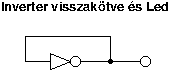
\includegraphics[scale=1.5]{dw/circuit_test4.pdf}
\vspace{-10pt}
\end{center}}
{Tesztelő}
{\vspace{-10pt}
\begin{itemize}
\setlength{\itemsep}{0cm}%
\setlength{\parskip}{0cm}%
\setlength{\itemindent}{-15pt}%
\item Áramkör és komponensek létrehozása
\item szimuláció indítása
\begin{itemize}
\setlength{\itemsep}{0cm}%
\setlength{\parskip}{0cm}%
\setlength{\itemindent}{-35pt}%
\item hálózat kiértékelés indítása
\begin{itemize}
\setlength{\itemsep}{0cm}%
\setlength{\parskip}{0cm}%
\setlength{\itemindent}{-50pt}%
	\item inverter kiértékelése
	\begin{itemize}
	\setlength{\itemsep}{0cm}%
	\setlength{\parskip}{0cm}%
	\setlength{\itemindent}{-65pt}%
		\item inverter bemenetének lekérdezése (\textbf{megkérdezi a tesztelőt}, javasolt: 0)
		\item inv. értékének kiadása a vezetékre (\textbf{megkérdezi a tesztelőt}, javasolt: 1)
	\end{itemize}
	\item node kiértékelése
	\begin{itemize}
	\setlength{\itemsep}{0cm}%
	\setlength{\parskip}{0cm}%
	\setlength{\itemindent}{-65pt}%
		\item node bemenetének lekérdezése (\textbf{megkérdezi a tesztelőt}, javasolt: 1)
		\item node értékének kiadása a vezetékekre (\textbf{megkérdezi a tesztelőt}, javasolt: mindkettőre 0)
	\end{itemize}
	\item led kiértékelése
	\begin{itemize}
	\setlength{\itemsep}{0cm}%
	\setlength{\parskip}{0cm}%
	\setlength{\itemindent}{-65pt}%
		\item led bemenetének lekérdezése (\textbf{megkérdezi a tesztelőt}, javasolt: 1)
	\end{itemize}
\end{itemize}
\item áramkör változásának vizsgálata
\begin{itemize}
\setlength{\itemsep}{0cm}%
\setlength{\parskip}{0cm}%
\setlength{\itemindent}{-50pt}%
	\item inverter változásának vizsgálata (\textbf{megkérdezi a tesztelőt}, javasolt: 1)
	\item led változásának vizsgálata (\textit{idáig nem kéne eljutni, ha fent jót válaszolt a tesztelő})
\end{itemize}
\item áramkör változott, ezért új ciklus
\item hálózat kiértékelés indítása
\begin{itemize}
\setlength{\itemsep}{0cm}%
\setlength{\parskip}{0cm}%
\setlength{\itemindent}{-50pt}%
	\item inverter kiértékelése
	\begin{itemize}
	\setlength{\itemsep}{0cm}%
	\setlength{\parskip}{0cm}%
	\setlength{\itemindent}{-65pt}%
		\item inverter bemenetének lekérdezése (\textbf{megkérdezi a tesztelőt}, javasolt: 1)
		\item inv. értékének kiadása a vezetékre (\textbf{megkérdezi a tesztelőt}, javasolt: 0)
	\end{itemize}
	\item node kiértékelése
	\begin{itemize}
	\setlength{\itemsep}{0cm}%
	\setlength{\parskip}{0cm}%
	\setlength{\itemindent}{-65pt}%
		\item node bemenetének lekérdezése (\textbf{megkérdezi a tesztelőt}, javasolt: 0)
		\item node értékének kiadása a vezetékekre (\textbf{megkérdezi a tesztelőt}, javasolt: mindkettőre 0)
	\end{itemize}
	\item led kiértékelése
	\begin{itemize}
	\setlength{\itemsep}{0cm}%
	\setlength{\parskip}{0cm}%
	\setlength{\itemindent}{-65pt}%
		\item led bemenetének lekérdezése (\textbf{megkérdezi a tesztelőt}, javasolt: 0)
	\end{itemize}
\end{itemize}
\item áramkör változásának vizsgálata
\begin{itemize}
\setlength{\itemsep}{0cm}%
\setlength{\parskip}{0cm}%
\setlength{\itemindent}{-50pt}%
	\item inverter változásának vizsgálata (\textbf{megkérdezi a tesztelőt}, javasolt: 1)
	\item led változásának vizsgálata (\textit{idáig nem kéne eljutni, ha fent jót válaszolt a tesztelő})
\end{itemize}
\item az áramkör ismét változott, nincs stacionárius állapota, szim. vége
\end{itemize}
\end{itemize}
\vspace{-15pt}}

\newpage

\usecase
{Kapcsoló, Vagy kapu visszakötve és Led}
{Ez a usecase egy olyan áramkör tesztelését mutatja be, amely egy kapcsolóból, egy VAGY kapuból, melynek egyik bemenetére a kapcsoló, másik bemenetére a saját kimenete van kötve és egy ledből, melyre szintén a VAGY kapu kimenetét kötöttük. Ez egy olyan visszakötéses hálózat, mely stabil állapotban van.
\newline
\begin{center}
\vspace{-15pt}
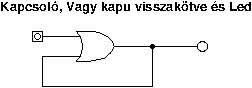
\includegraphics[scale=1.5]{dw/circuit_test5.pdf}
\vspace{-10pt}
\end{center}}
{Tesztelő}
{\vspace{-15pt}
\begin{itemize}
\setlength{\itemsep}{0cm}%
\setlength{\parskip}{0cm}%
\setlength{\itemindent}{-15pt}%
\item Áramkör és komponensek létrehozása
\item szimuláció indítása
\begin{itemize}
\setlength{\itemsep}{0cm}%
\setlength{\parskip}{0cm}%
\setlength{\itemindent}{-35pt}%
\item hálózat kiértékelés indítása
\begin{itemize}
\setlength{\itemsep}{0cm}%
\setlength{\parskip}{0cm}%
\setlength{\itemindent}{-50pt}%
	\item kapcsoló kiértékelése
	\begin{itemize}
	\setlength{\itemsep}{0cm}%
	\setlength{\parskip}{0cm}%
	\setlength{\itemindent}{-65pt}%
		\item kapcsoló állapotának lekérdezése (\textbf{megkérdezi a tesztelőt}, javasolt: 1)
		\item kapcsoló értékének kiadása a vezetékre
	\end{itemize}
	\item kapu kiértékelése
	\begin{itemize}
	\setlength{\itemsep}{0cm}%
	\setlength{\parskip}{0cm}%
	\setlength{\itemindent}{-65pt}%
		\item kapu egyik bemenetének (amelyiken a kapcsoló van) lekérdezése (\textbf{megkérdezi a tesztelőt}, javasolt: 1)
		\item kapu másik bemenetének lekérdezése (\textbf{megkérdezi a tesztelőt}, javasolt: 0)
		\item kapu értékének kiadása a vezetékre (\textbf{megkérdezi a tesztelőt}, javasolt: 1)
	\end{itemize}
	\item led kiértékelése
	\begin{itemize}
	\setlength{\itemsep}{0cm}%
	\setlength{\parskip}{0cm}%
	\setlength{\itemindent}{-65pt}%
		\item led bemenetének lekérdezése (\textbf{megkérdezi a tesztelőt}, javasolt: 1)
	\end{itemize}
\end{itemize}
\item áramkör változásának vizsgálata
\begin{itemize}
\setlength{\itemsep}{0cm}%
\setlength{\parskip}{0cm}%
\setlength{\itemindent}{-50pt}%
	\item kapcsoló változásának vizsgálata (\textbf{megkérdezi a tesztelőt}, javasolt: 1)
	\item kapu változásának vizsgálata (\textit{idáig nem kéne eljutni, ha fent jót válaszolt a tesztelő})
	\item led változásának vizsgálata (\textit{idáig nem kéne eljutni, ha fent jót válaszolt a tesztelő})
\end{itemize}
\item áramkör változott, ezért új ciklus
\item hálózat kiértékelés indítása
\begin{itemize}
\setlength{\itemsep}{0cm}%
\setlength{\parskip}{0cm}%
\setlength{\itemindent}{-50pt}%
	\item kapcsoló kiértékelése
	\begin{itemize}
	\setlength{\itemsep}{0cm}%
	\setlength{\parskip}{0cm}%
	\setlength{\itemindent}{-65pt}%
		\item kapcsoló állapotának lekérdezése (\textbf{megkérdezi a tesztelőt}, javasolt: 1)
		\item kapcsoló értékének kiadása a vezetékre
	\end{itemize}
	\item kapu kiértékelése
	\begin{itemize}
	\setlength{\itemsep}{0cm}%
	\setlength{\parskip}{0cm}%
	\setlength{\itemindent}{-65pt}%
		\item kapu egyik bemenetének (amelyiken a kapcsoló van) lekérdezése (\textbf{megkérdezi a tesztelőt}, javasolt: 1)
		\item kapu másik bemenetének lekérdezése (\textbf{megkérdezi a tesztelőt}, javasolt: 1)
		\item kapu értékének kiadása a vezetékre (\textbf{megkérdezi a tesztelőt}, javasolt: 1)
	\end{itemize}
	\item led kiértékelése
	\begin{itemize}
	\setlength{\itemsep}{0cm}%
	\setlength{\parskip}{0cm}%
	\setlength{\itemindent}{-65pt}%
		\item led bemenetének lekérdezése (\textbf{megkérdezi a tesztelőt}, javasolt: 1)
	\end{itemize}
\end{itemize}
\item áramkör változásának vizsgálata
\begin{itemize}
\setlength{\itemsep}{0cm}%
\setlength{\parskip}{0cm}%
\setlength{\itemindent}{-50pt}%
	\item kapcsoló változásának vizsgálata (\textbf{megkérdezi a tesztelőt}, javasolt: 0)
	\item kapu változásának vizsgálata (\textbf{megkérdezi a tesztelőt}, javasolt: 0)
	\item led változásának vizsgálata (\textbf{megkérdezi a tesztelőt}, javasolt: 0)
\end{itemize}
\item áramkör nem változott, stabil állapot
\item FF-okat véglegesítjük (nem történik semmi, mert nincs FF)
\item jelgenerátorokat léptetjük (nem történik semmi, mert nincs jelgenerátor)
\item stacionárius állapot, szimuláció vége
\end{itemize}
\end{itemize}
\vspace{-15pt}}

\section{Architektúra}

\section{A szkeleton kezelői felületének terve, dialógusok}
Az általunk elkészített szkeleton egy program váz melynek felülete egy egyszerű konzolos megjelenítési felület, amely alkalmas arra, hogy a use case-k által leírt teszteseteket bemutassuk. Az egyes tesztesetek a neki megfelelő use case sorszámával van elnevezve, így program indítás után egy szám bevitelét követően a kiválasztott teszteset lefut. 
A teszteset futása közben kiír minden objektumot amin metódust hív, illetve kiírja a metódus nevét a paraméterekkel együtt, majd a visszatérési értéket. Ez azért lehetséges, mert a szkeleton már tartalmazza az elkészítendő szoftver összes fontos osztályát és metódusát, azonban az üzleti logikát még nem. Így könnyen eldönthető, hogy a use case-nek megfelelően viselkedik a program és továbbiakban képes lesz-e megfelelően működni.
A tesztelési folyamat során döntési helyzet léphet fel. Ilyenkor a program felteszi a kérdést, majd a kapott válasz alapján folytatja a további futást. Ezzel csökkentjük a tesztesetek számát, anélkül, hogy bizonyos esetek kimaradnának a tesztelés alól. 
Futás közben megjegyzés formájában a program tájékoztat néhány elem valamilyen tulajdonságáról (például az adott bemenet miatt a kijelző világít, vagy nem) vagy bizonyos fontosabb lépésekről (például inicializálás).
Az elvárás, hogy a szkeleton a szekvenciadiagramok által leírt működést mutassa. A program egyszerű és könnyen összehasonlítható formában írja ki a működését, amelyet könnyen összevethetjük a szekvencia diagrammokkal.

\subsection{Program üzeneteinek formátuma}

A program a következő eseményeket jelzi ki:
\begin{itemize}
\item Konstruktor hívás.\\
	  Formátum: \texttt{CREATE osztálynév objektumnév}\\
	  Példa: \texttt{CREATE Circuit circuit}
\item Tagfüggvény hívás.\\
	  Formátum: \texttt{CALL objektumnév.metódus(paraméterek)}\\
	  Példa: \texttt{CALL wire.setValue(Value.TRUE)}
\item Konstruktor/tagfüggvény visszatér\\
	  Formátum: \texttt{RETURN} vagy \texttt{RETURN objektumnév/érték}\\
	  Ha van visszatérési érték az kétféle lehet: referencia valamelyik objektumra (ekkor az objektumnevet írjuk ki), vagy egy konkrét érték (ilyenkor az értéket, pl: \texttt{false}).
\item Kérdés a felhasználónak.\\
	  Formátum: \texttt{QUESTION objektumnév üzenet? [opciók]}\\
	  Példa: \texttt{QUESTION wire vezetéken lévő érték? [0/1]}\\
	  Objektumnév annak az objektumnak a neve, aki kérdezi a felhasználót. Az opciókban lévő elemek \texttt{/} jellel vannak elválasztva. Addig nem megy tovább a program, amíg nem ezek közül kap választ.
\item Megjegyzés kijelzése.\\
	Formátum: \texttt{\# üzenet}
\end{itemize}

Formátum bemutatásához egy összetettebb példa:

\begin{verbatim}
CALL simulation.start()
  CALL circuit.doEvaluationCycle()
    CALL toggle.evaluate()
      QUESTION toggle állapot? [0/1] 1
      CALL wire.setValue(Value.TRUE)
      RETURN
    RETURN
    CALL led.evaluate()
      CALL wire.getValue()
        QUESTION wire vezetéken lévő érték? [0/1] 1
      RETURN Value.TRUE
    RETURN
  RETURN
  CALL circuit.isChanged()
    CALL toggle.isChanged()
      QUESTION toggle változott? [0/1] 1
    RETURN true
  RETURN true
  CALL circuit.doEvaluationCycle()
    CALL toggle.evaluate()
      QUESTION toggle állapot? [0/1] 1
      CALL wire.setValue(Value.TRUE)
      RETURN
    RETURN
    CALL led.evaluate()
      CALL wire.getValue()
        QUESTION wire vezetéken lévő érték? [0/1] 1
      RETURN Value.TRUE
    RETURN
  RETURN
  CALL circuit.isChanged()
    CALL toggle.isChanged()
      QUESTION toggle változott? [0/1] 0
    RETURN false
    CALL led.isChanged()
      QUESTION led változott? [0/1] 0
    RETURN false
  RETURN false
  CALL circuit.commitFlipFlops()
  RETURN
  CALL circuit.stepGenerators()
  RETURN
RETURN true
\end{verbatim}

\section{Szekvencia diagramok a belső működésre}

\begin{figure}[H]
\begin{center}
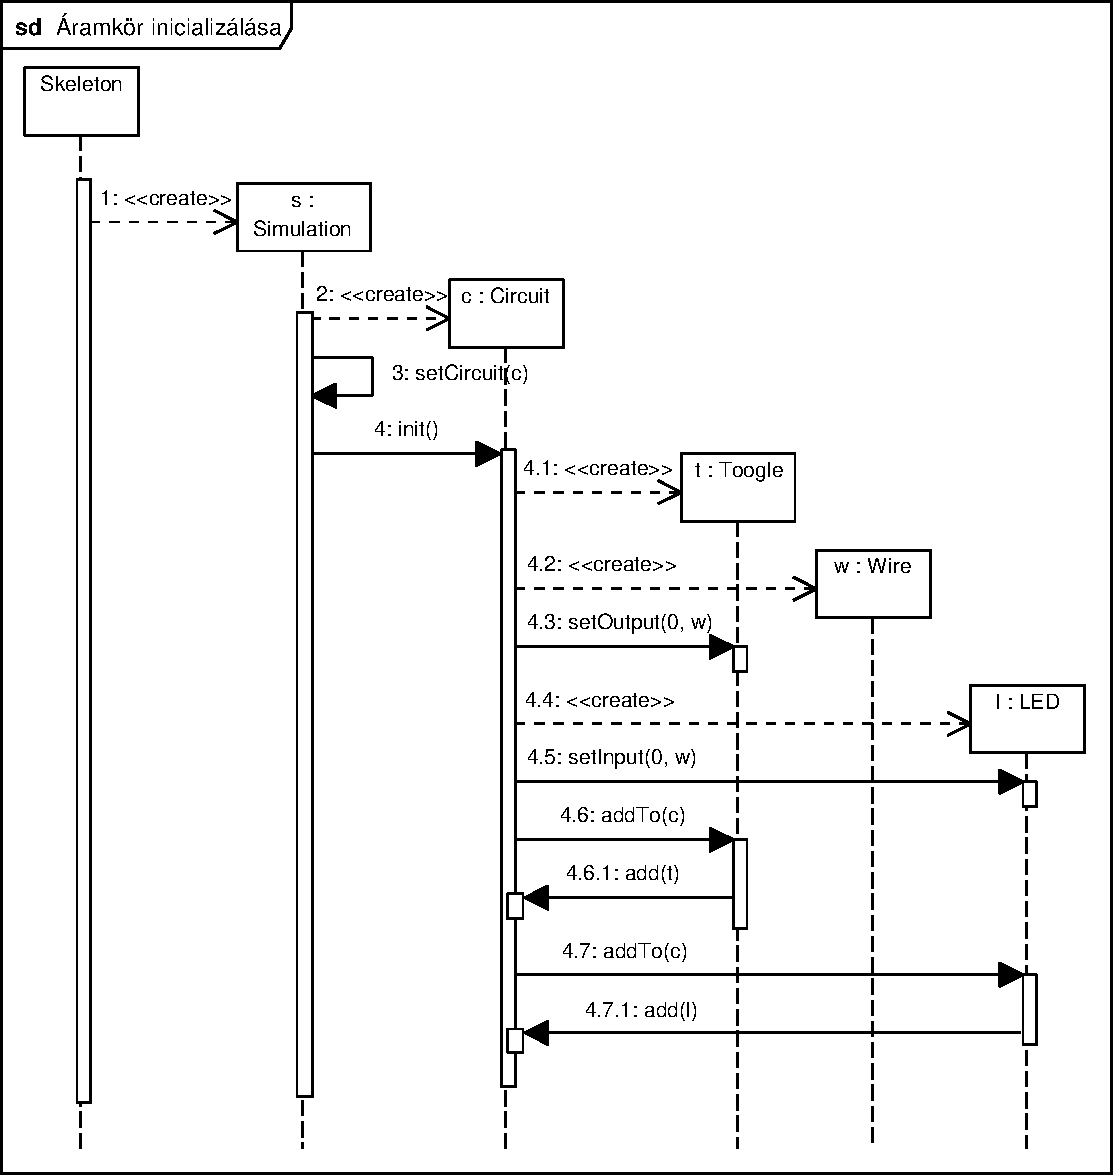
\includegraphics[width=17cm]{chapters/chapter05/imgs/init.pdf}
\caption{Áramkör inicializálása}
\label{fig:init}
\end{center}
\end{figure}

\begin{figure}[H]
\begin{center}
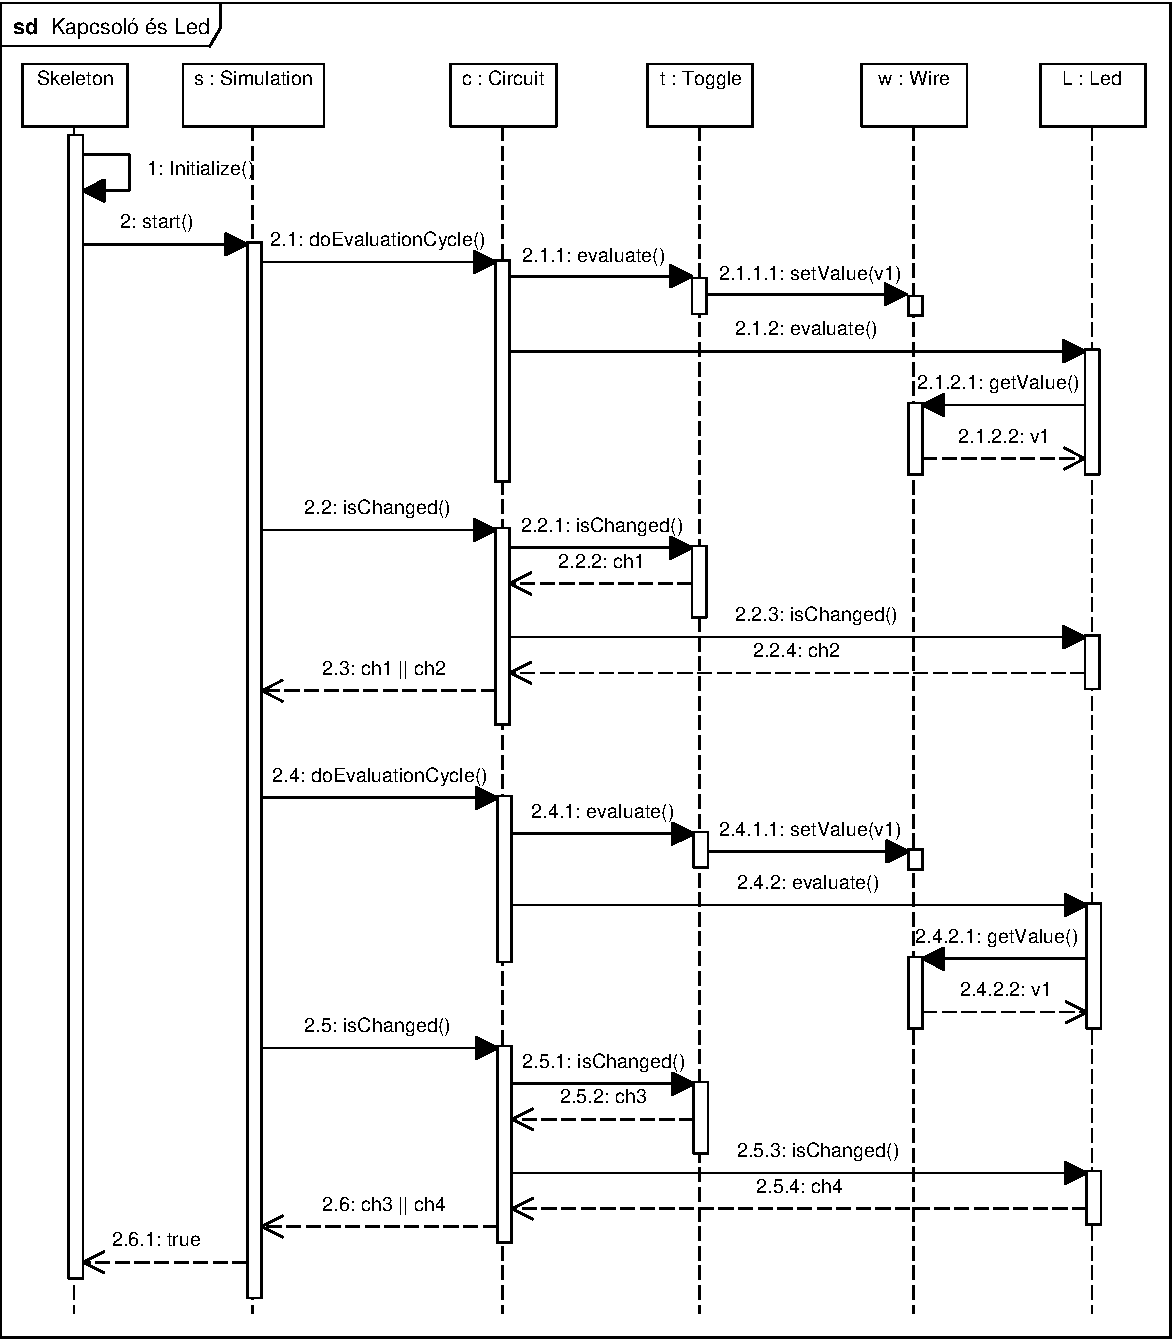
\includegraphics[width=17cm]{chapters/chapter05/imgs/test1.pdf}
\caption{Kapcsoló és Led}
\label{fig:test1}
\end{center}
\end{figure}

\begin{figure}[H]
\begin{center}
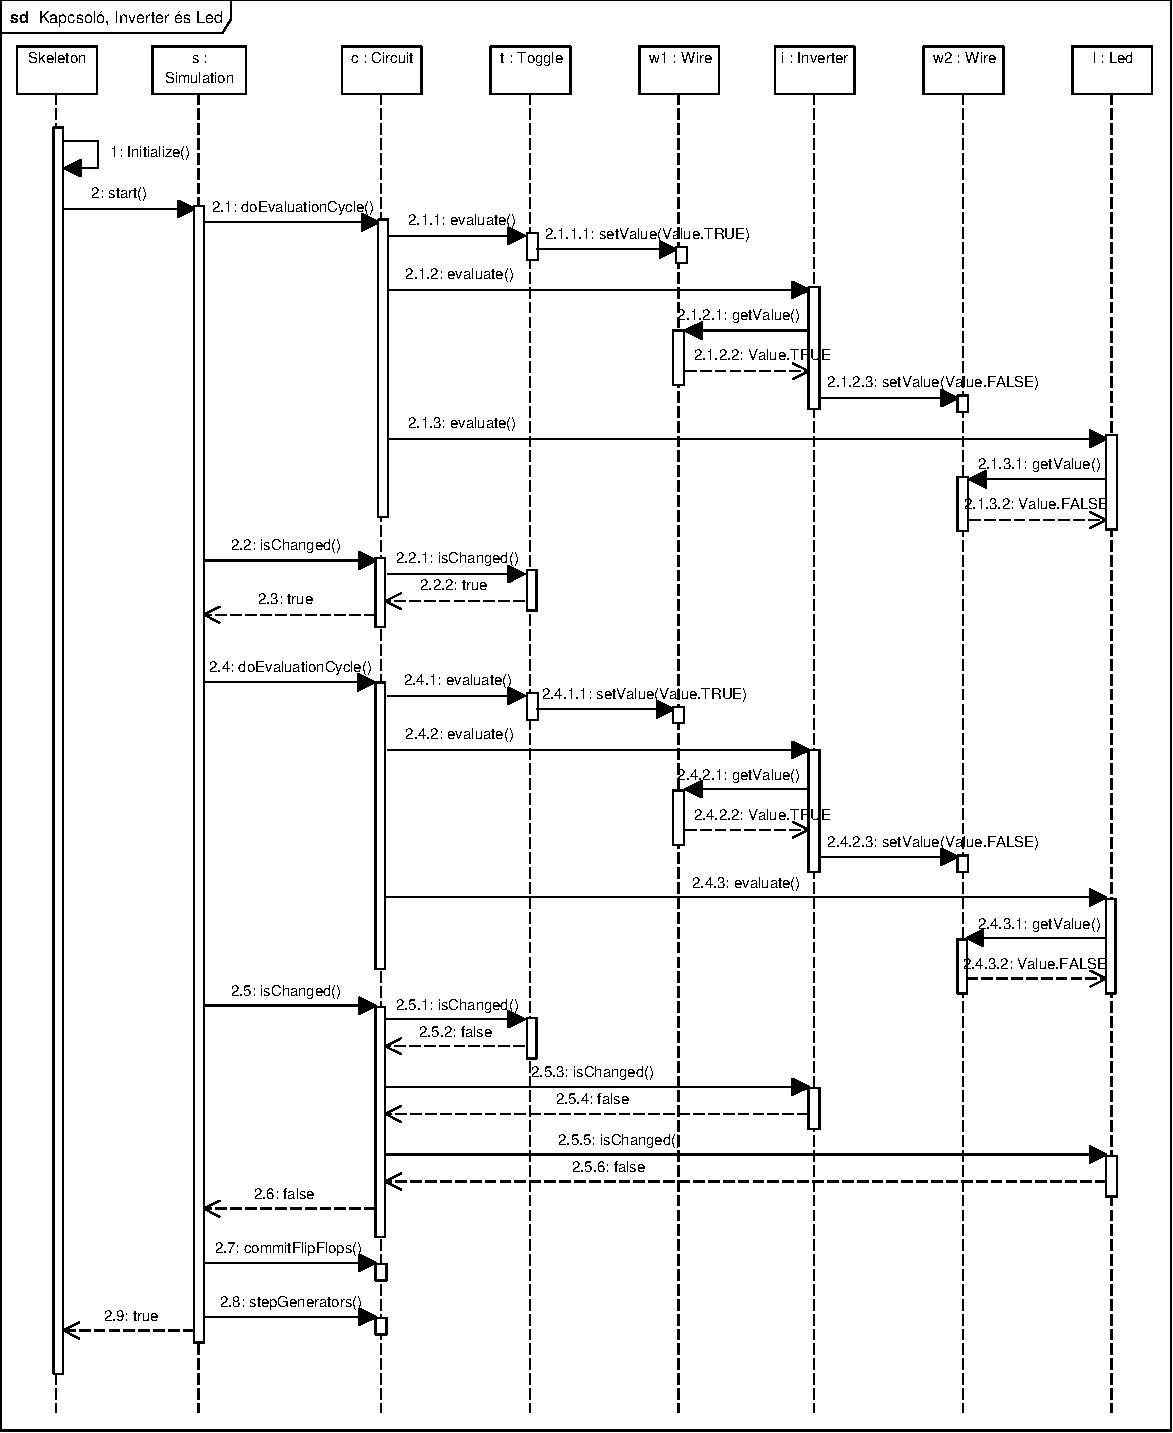
\includegraphics[width=17cm]{chapters/chapter05/imgs/test2.pdf}
\caption{Kapcsoló, Inverter és Led}
\label{fig:test2}
\end{center}
\end{figure}

\begin{figure}[H]
\begin{center}
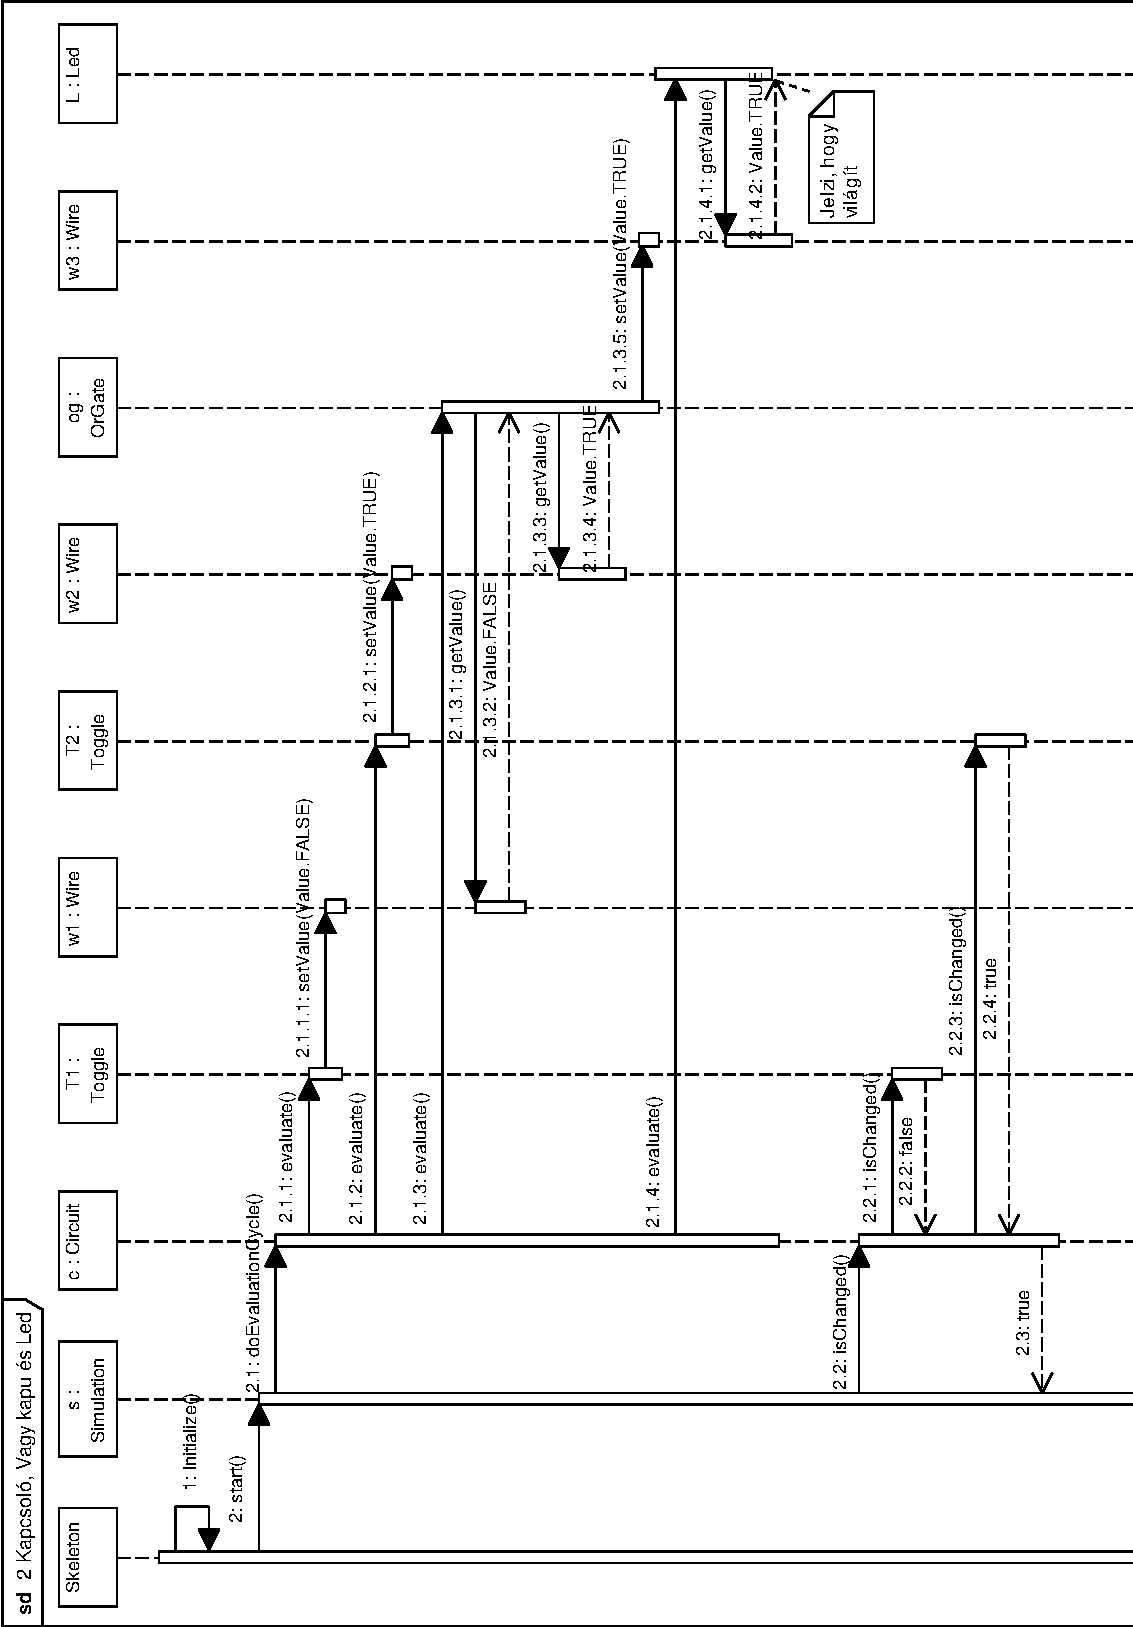
\includegraphics[width=16cm]{chapters/chapter05/imgs/test3-1.pdf}
\caption{2 Kapcsoló, Vagy kapu és Led (1. rész)}
\label{fig:test3_1}
\end{center}
\end{figure}

\begin{figure}[H]
\begin{center}
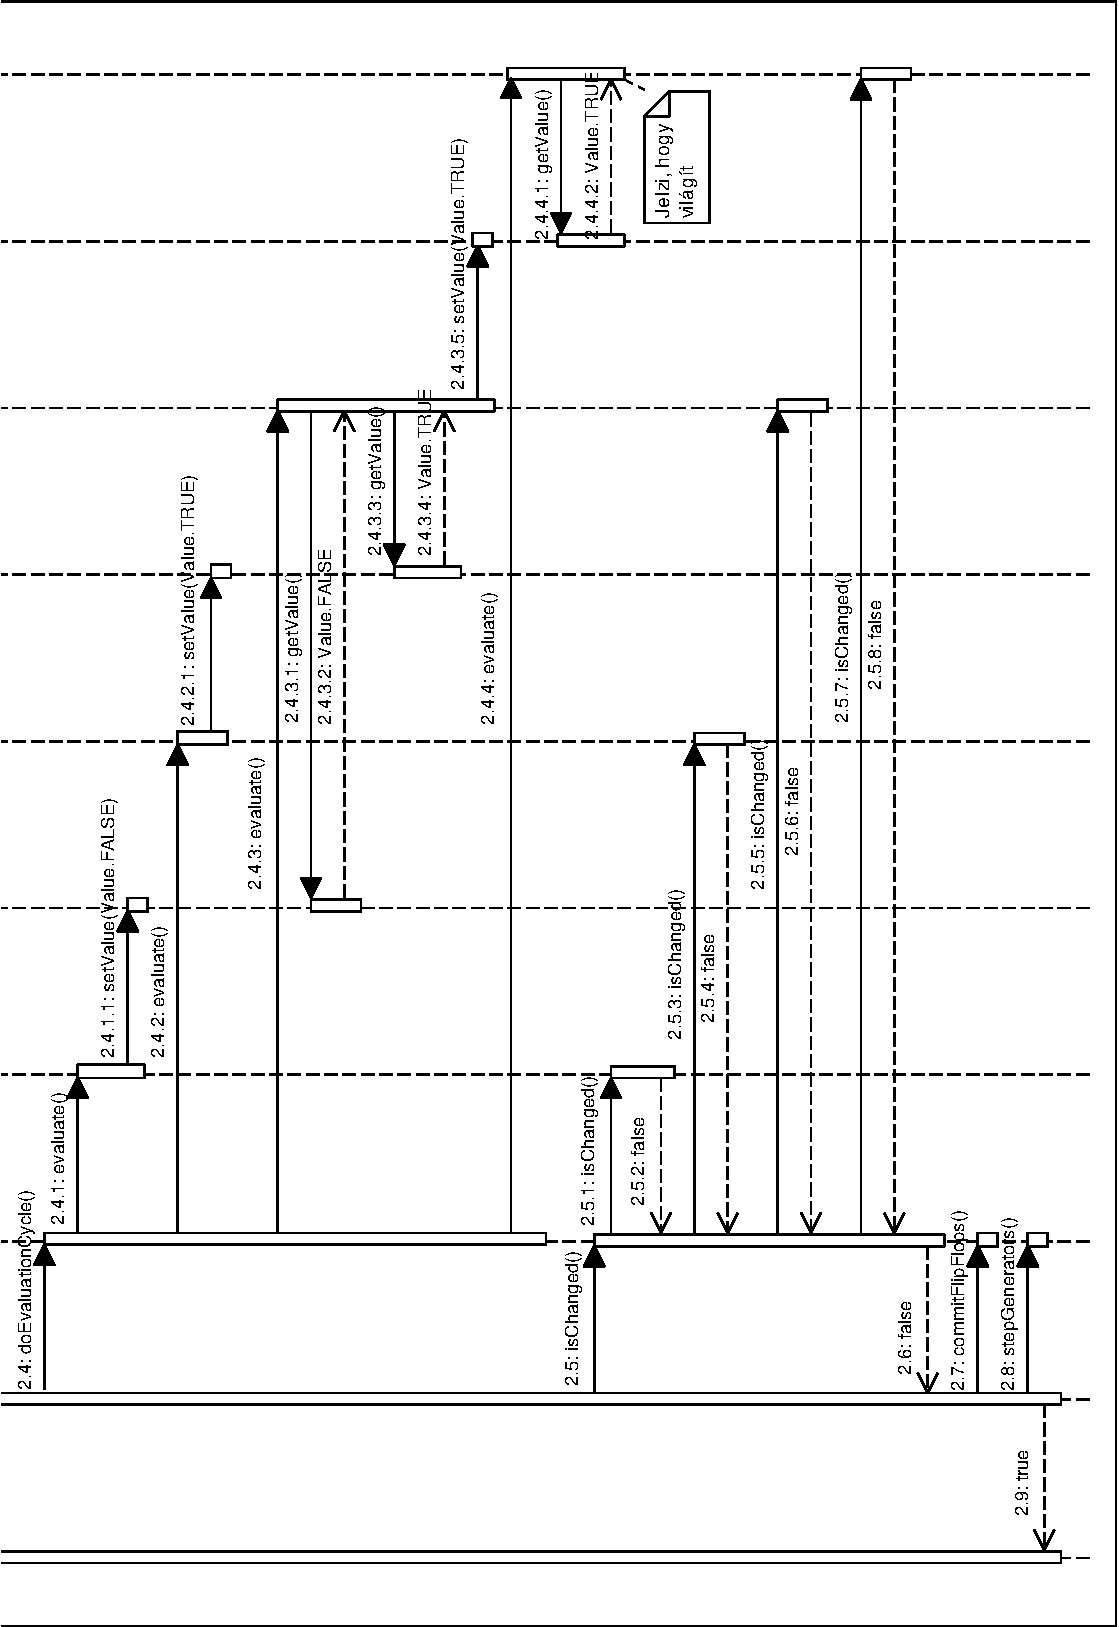
\includegraphics[width=16cm]{chapters/chapter05/imgs/test3-2.pdf}
\caption{2 Kapcsoló, Vagy kapu és Led (2. rész)}
\label{fig:test3_2}
\end{center}
\end{figure}

\begin{figure}[H]
\begin{center}
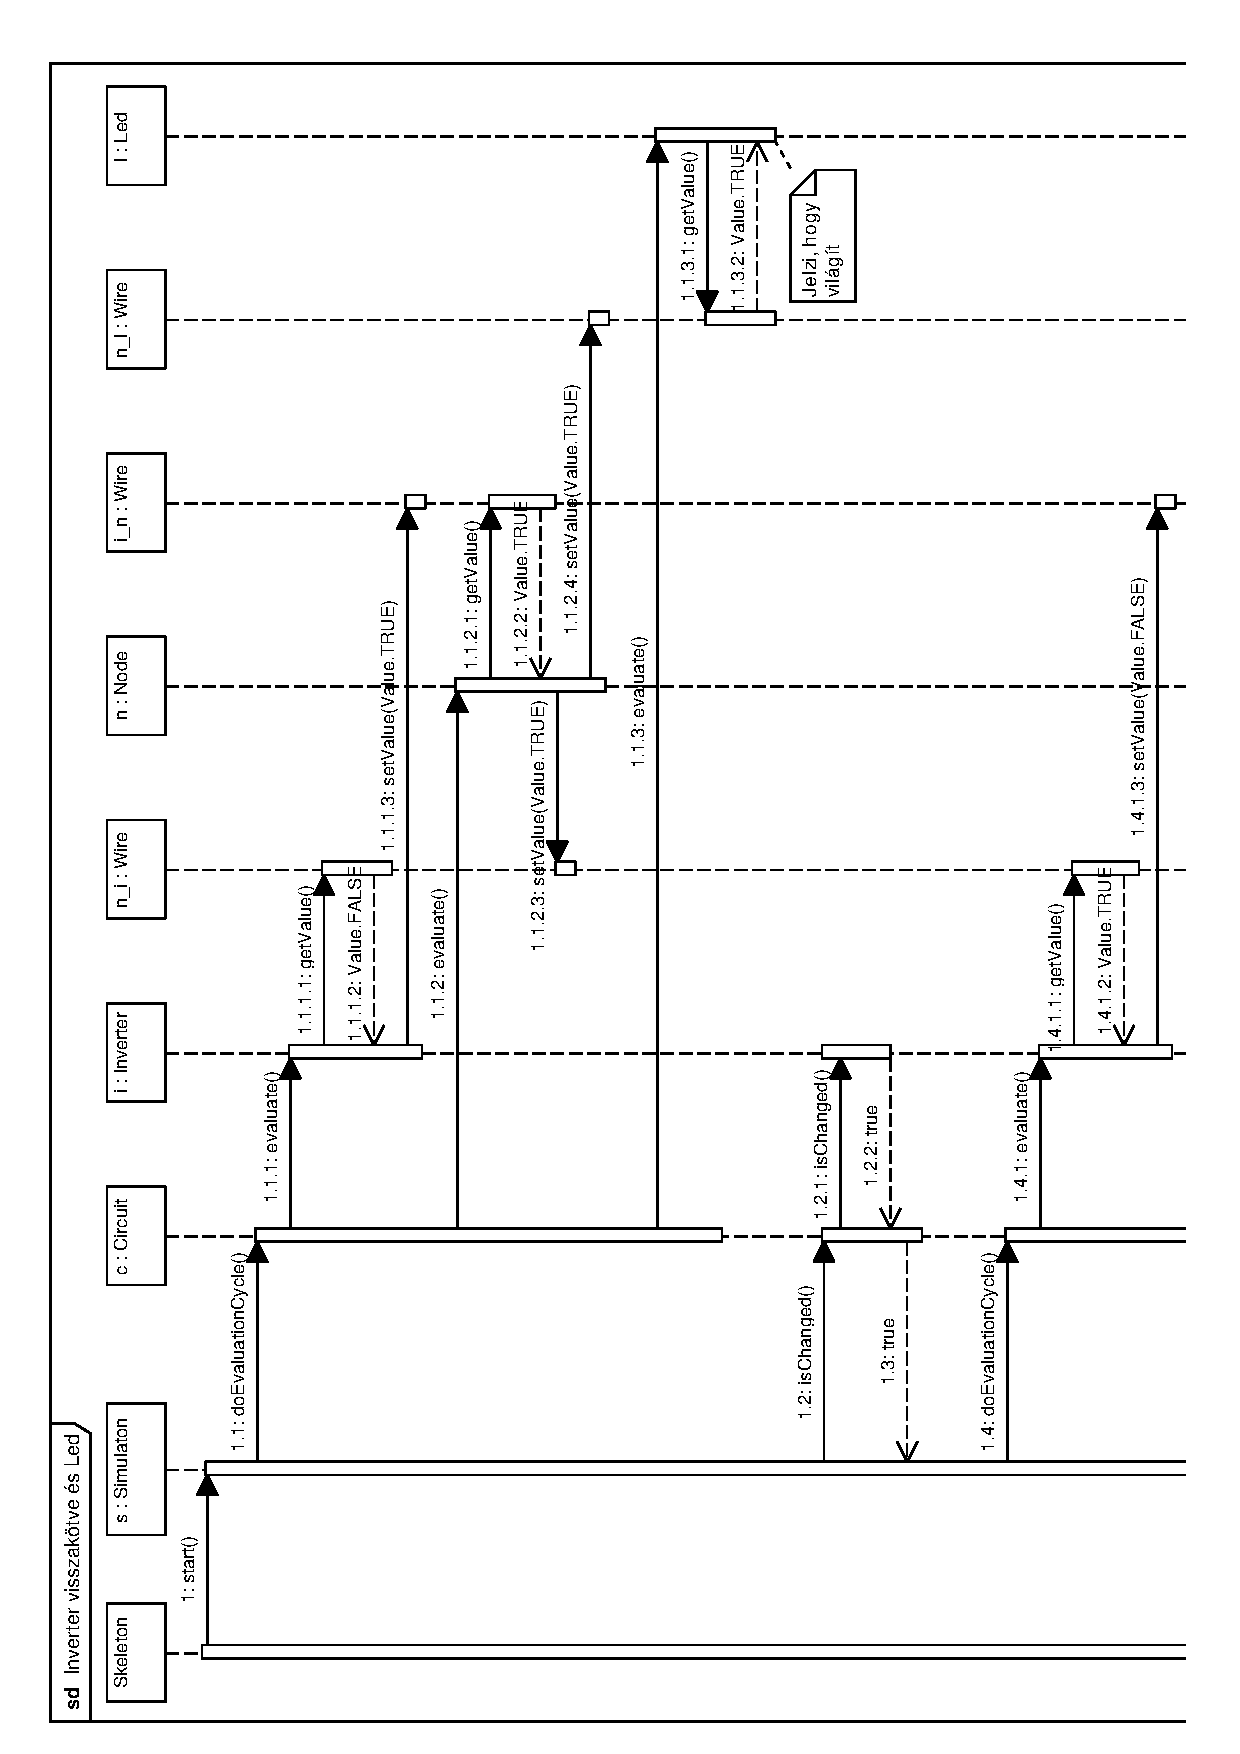
\includegraphics[height=23cm]{chapters/chapter05/imgs/test4-1.pdf}
\caption{Inverter visszakötve és Led (1. rész)}
\label{fig:test4_1}
\end{center}
\end{figure}

\begin{figure}[H]
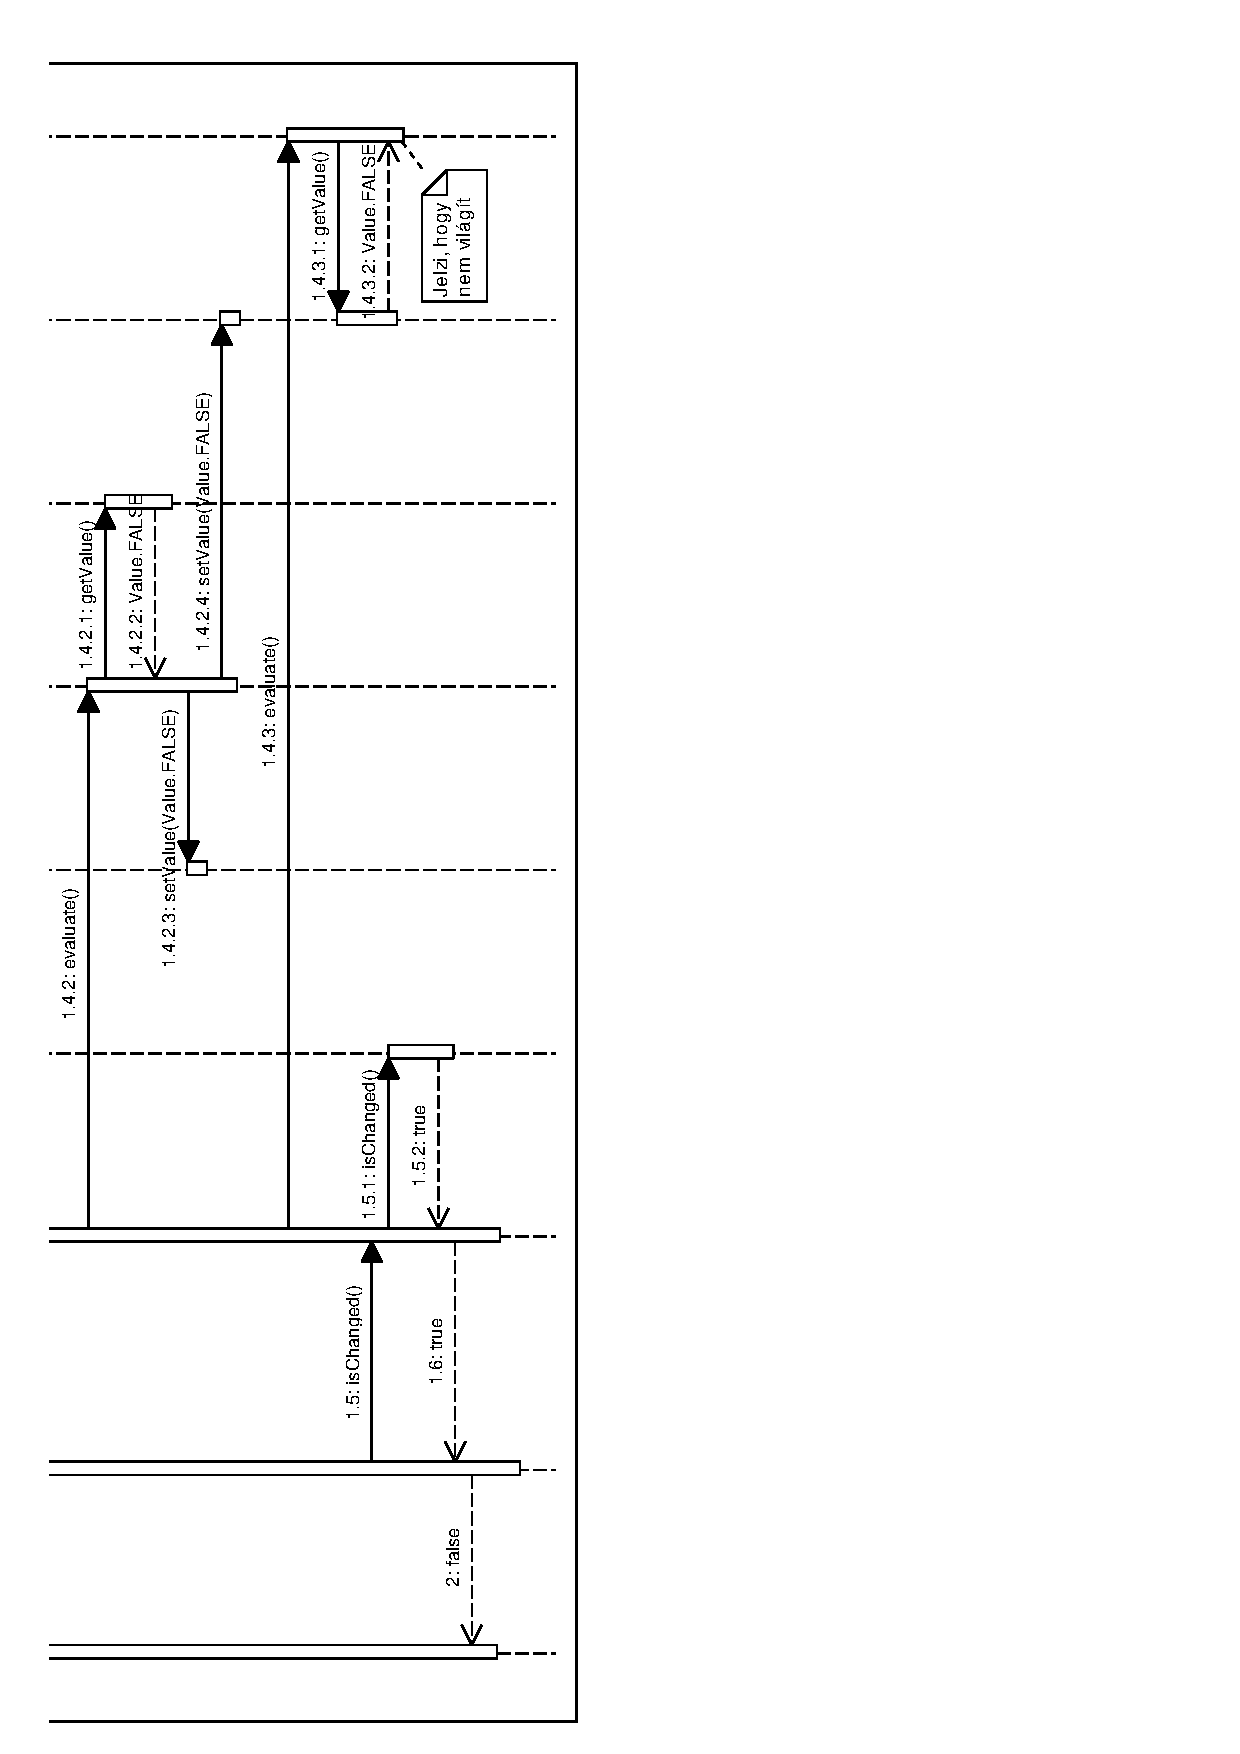
\includegraphics[height=23cm]{chapters/chapter05/imgs/test4-2.pdf}
\caption{Inverter visszakötve és Led (2. rész)}
\label{fig:test4_2}
\end{figure}


\begin{figure}[H]
\begin{center}
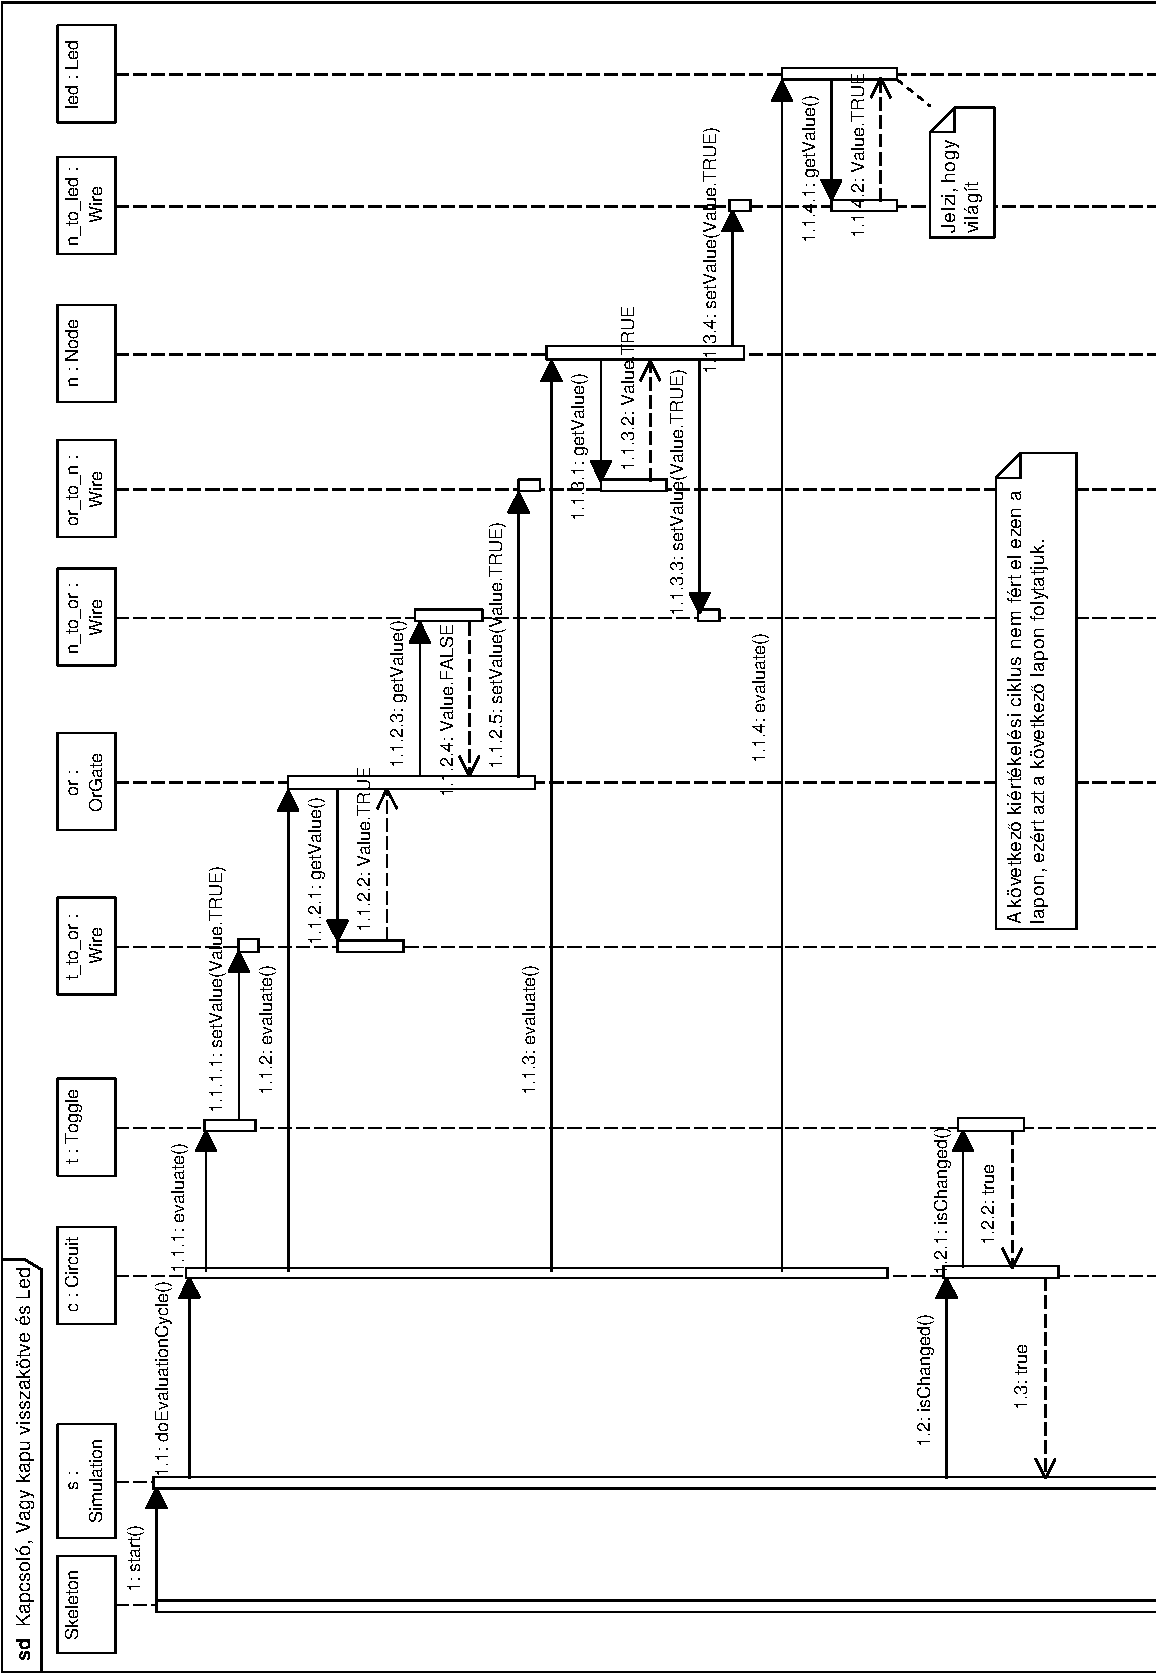
\includegraphics[width=16cm]{chapters/chapter05/imgs/test5-1.pdf}
\caption{Kapcsoló, Vagy kapu visszakötve és Led (1. rész)}
\label{fig:test5_1}
\end{center}
\end{figure}

\begin{figure}[H]
\begin{center}
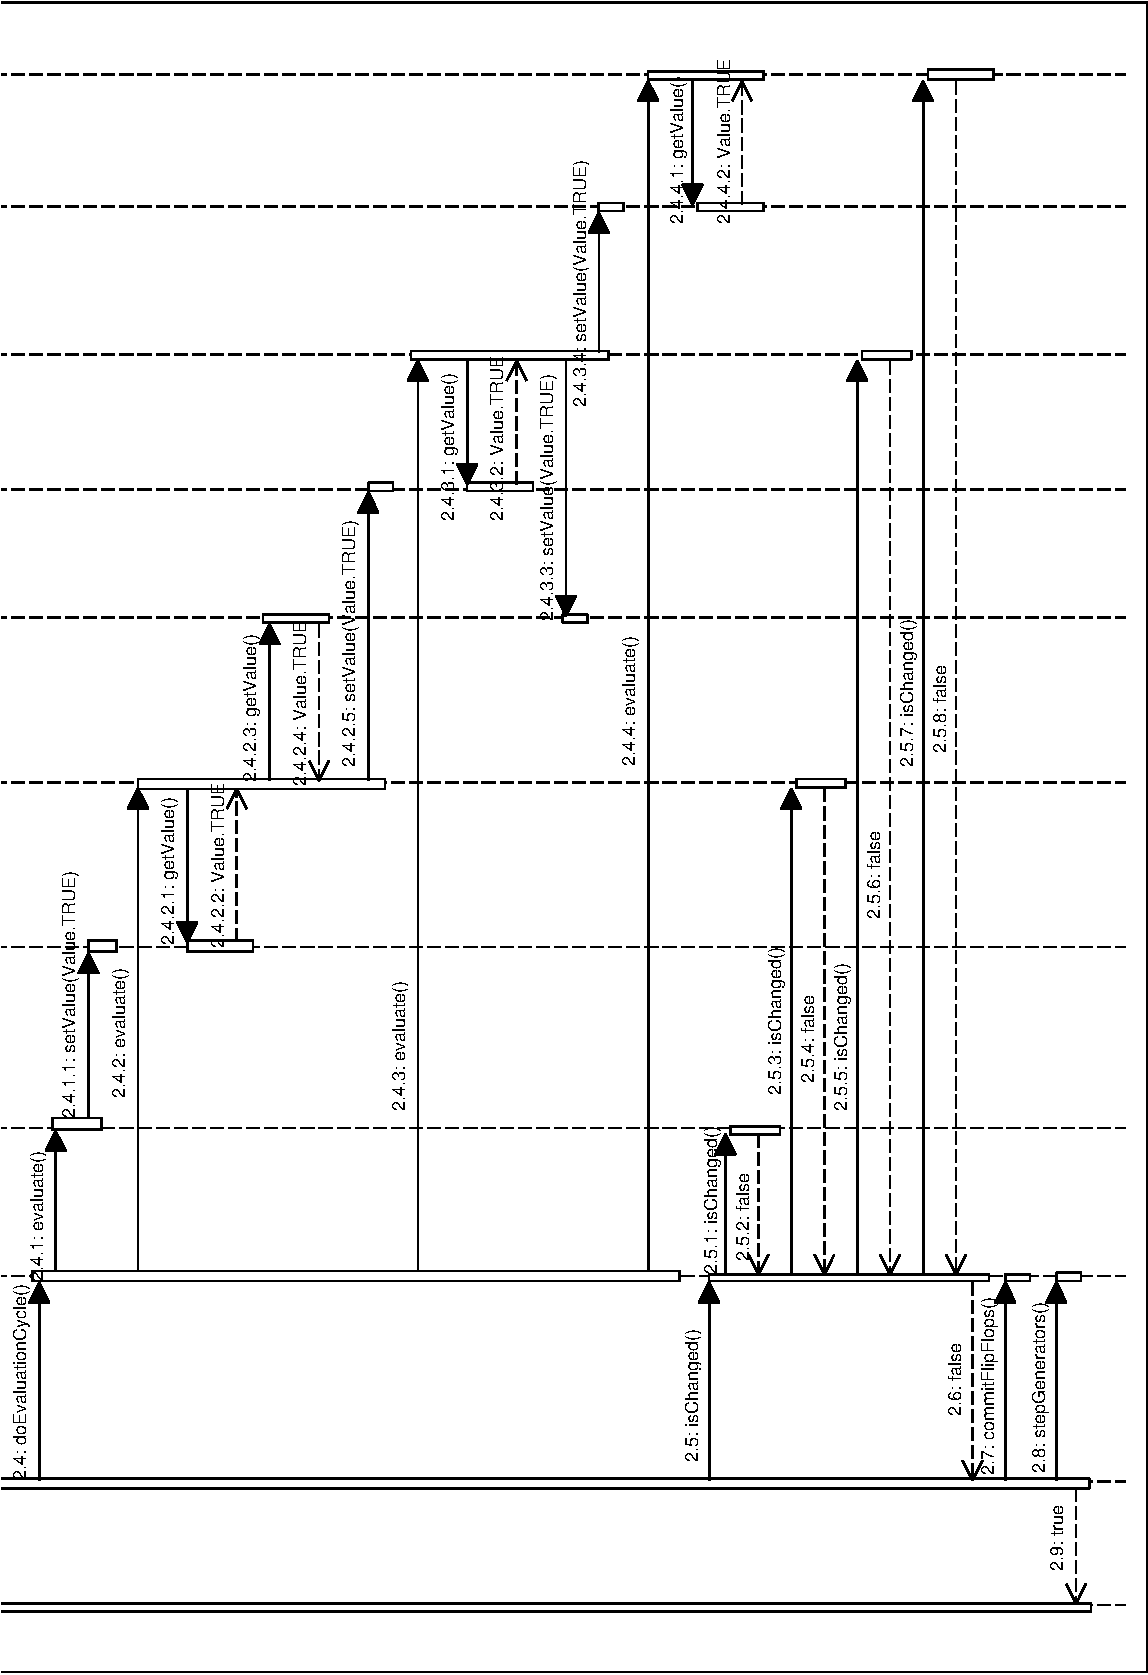
\includegraphics[width=16cm]{chapters/chapter05/imgs/test5-2.pdf}
\caption{Kapcsoló, Vagy kapu visszakötve és Led (2. rész)}
\label{fig:test5_2}
\end{center}
\end{figure}